% Michael Baudin, 2017 - 2019
\documentclass{article}

% Copyright (C) 2012 - 2013 - EDF R&D - Michael Baudin

\setbeameroption{hide notes}
%\setbeameroption{show notes}
%\setbeameroption{show only notes}
%\mode<presentation>{\usetheme{EDF09}}

% Configuration beamer
\usetheme{Montpellier}
\setbeamertemplate{navigation symbols}{} % Remove navigation
\useoutertheme{infolines}
\setbeamertemplate{theorems}[numbered] 
% Utilise des fonts serif, pour �viter les pb de fonte
\usefonttheme{serif} 
\setbeamertemplate{caption}[numbered]


\usepackage[utf8]{inputenc}
\usepackage[T1]{fontenc}


\usepackage[french]{babel}
\uselanguage{French}
\languagepath{French}

% Scilab macros
\newcommand{\sciobj}[1]{\texttt{#1}}
\newcommand{\scifile}[1]{\texttt{#1}}

% Python macros
\newcommand{\pyobj}[1]{\textcolor{blue}{\texttt{#1}}}

\def\RR{\mathbb{R}}
\def\NN{\mathbb{N}}
\def\ZZ{\mathbb{Z}}
\def\bx{{\bf x}}

% To highlight source code
\usepackage{listingsutf8}
\lstset{inputencoding=utf8/latin1}

\definecolor{darkgreen}{rgb}{0,0.5,0}
\definecolor{violet}{rgb}{0.5,0,1}
\lstset{
  % general command to set parameter(s)
   basicstyle=\scriptsize\ttfamily, %
   keywordstyle=\color{violet}\bfseries,%
   commentstyle=\color{darkgreen}\bfseries,%
   showspaces=false,%
   stringstyle=\color{red}\bfseries
}

\hypersetup{
    %bookmarks=true,         % show bookmarks bar?
    %unicode=false,          % non-Latin characters in Acrobat�s bookmarks
    %pdftoolbar=true,        % show Acrobat�s toolbar?
    %pdfmenubar=true,        % show Acrobat�s menu?
    %pdffitwindow=false,     % window fit to page when opened
    %pdfstartview={FitH},    % fits the width of the page to the window
    %pdftitle={My title},    % title
    %pdfauthor={Author},     % author
    %pdfsubject={Subject},   % subject of the document
    %pdfcreator={Creator},   % creator of the document
    %pdfproducer={Producer}, % producer of the document
    %pdfkeywords={keyword1} {key2} {key3}, % list of keywords
    %pdfnewwindow=true,      % links in new window
    colorlinks=true,       % false: boxed links; true: colored links
    %linkcolor=red,          % color of internal links (change box color with linkbordercolor)
    %citecolor=green,        % color of links to bibliography
    %filecolor=magenta,      % color of file links
    urlcolor=blue           % color of external links
}

%%%%%%%%%%%%%%%%%%%%%%%%%%%%%%%%%%%%%%%%%%%%%%%%%%%%%%%%%%%%%%%%%%%

\begin{document}


\title{OpenTURNS and its graphical interface}

\author[1]{Michaël Baudin}
\author[1]{Anne Dutfoy}
\author[1]{Anthony Geay}
\author[1]{Thibault Delage}
\author[2]{Aurélie Ladier}
\author[2]{Julien Schueller}
\author[2]{Thierry Yalamas}
\affil[1]{Phimeca Engineering. 18/20 boulevard de Reuilly, 75012 Paris - France, yalamas@phimeca.com}
\affil[2]{EDF R\&D. 6, quai Watier, 78401, Chatou Cedex - France, michael.baudin@edf.fr}

\maketitle


\abstract{
OpenTURNS is an open source library for uncertainty propagation by 
probabilistic methods. 
Developed in a partnership of five industrial companies (EDF, Airbus, 
Phimeca, IMACS and ONERA), it benefits from a strong practical feedback. 
Classical algorithms of UQ are available : central dispersion, 
probability of exceedance, sensitivity analysis, metamodels and 
stochastic processes. 
Developed in C++, OpenTURNS is also available as a Python module and 
has gained maturity thanks to more than 10 years of development. 

However, there are situations where the engineer in charge of 
performing an uncertainty study does not want to use a programming 
language such as C++ or Python. 
In this context, providing a graphical user interface (GUI) may allow 
to greatly increase the use of OpenTURNS and, more generally, of the 
UQ methodology. 

In this paper, we present a basic tutorial of OpenTURNS in Python 
and will review the new features in the library, which include 
new incremental statistical estimators. 
In the second part, we review the new features in the open source GUI will be 
presented, including the management of stochastic processes. 
}

\tableofcontents

%%%%%%%%%%%%%%%%%%%%%%%%%%%%%%%%%%%%%%%%%%%%%%%%%

\section{Introduction}

OpenTURNS is a C++ library for uncertainty propagation by probabilistic 
methods. 
OpenTURNS is also available as a Python module and has gained maturity thanks to more 
than 10 years of development. 
However, there are situations where the engineer in charge of 
performing an uncertainty study does not want to use a programming language such as C++, Python 
(e.g. OpenTURNS) or Matlab. 
In this context, providing a graphical user interface (GUI) may allow 
to increase the use of OpenTURNS and, more generally, of the UQ methodology.

%%%%%%%%%%%%%%%%%%%%%%%%%%%%%%%%%%%%%%%%%%%%%%%%%


\section{OpenTurns}

OpenTURNS\cite{Baudin2016,OTurl,OpenTURNSUncecomp17} is an open source software, available as a 
C++ library and a Python interface. 
It works under the Linux and Windows environments. 
The key features of OpenTURNS are the following:
\begin{itemize}
\item open source initiative to secure the transparency of the approach,
\item generic to the physical or industrial domains for treating of multi-physical problems,
\item high performance computing,
\item includes a variety of qualified algorithms in order to manage uncertainties in several situations,
\item contains complete documentation (Reference Guide, Use Cases Guide, User manual, Examples Guide, and Developers' Guide).
\end{itemize}
OpenTURNS is available under the LGPL license. 

The main features of OpenTURNS are uncertainty quantification, uncertainty propagation, 
sensitivity analysis and metamodeling. 

Moreover generic wrappers allows to link OpenTURNS to any external code G.

OpenTURNS can be downloaded from its dedicated website www.openturns.org which offers different 
pre-compiled packages specific to several Windows and Linux environments. It is also possible to 
download the source files from the SourceForge server and to compile them within another 
environment: the OpenTURNS Developer's Guide provides advices to help compiling the source files.

%%%%%%%%%%%%%%%%%%%%%%%%%%%%%%%%%%%%%%%%%%%%%%%%%

\section{A tutorial example : the flooding model}

\subsection{Introduction}

In this paper, we illustrate our discussion with a simple application model that simulates 
the height of a river. 
The figure \ref{fig:crues} presents the dyke that protects industrial facilities. 
When the river height exceeds the one of the dyke, flooding occurs. 
This academic model is used as a pedagogical example in \cite{ioolem15}.
The model is based on a crude simplification of the 1D hydro-dynamical equations of SaintVenant 
under the assumptions of uniform and constant flowrate and large rectangular sections. 
It consists of an equation that involves the characteristics of the river stretch:
\begin{equation}\label{eq:cruesS}
S = Z_v + H \quad \mbox{with} \quad 
H = \left(\frac{Q}{B K_s \sqrt{\frac{Z_m-Z_v}{L} }} \right)^{0.6},
\end{equation}
where $S$ is the maximal annual overflow, $H$ is the maximal annual height of the river, 
$B$ is the river width and $L$ is the length of the river stretch. 
In this paper, we set the values of $L$ and $B$ parameters :
$$
L = 5000 \quad B = 300.
$$
The other four input variables $Q$, $K_s$, $Z_v$ and $Z_m$ are defined in Table \ref{tab:factors} 
with their  probability distribution.
The randomness of these variables is due to their spatio-temporal variability, our ignorance of 
their true value or some inaccuracies of their estimation. 
We make the hypothesis that the input variables are independent.

\begin{figure}
\begin{center}
    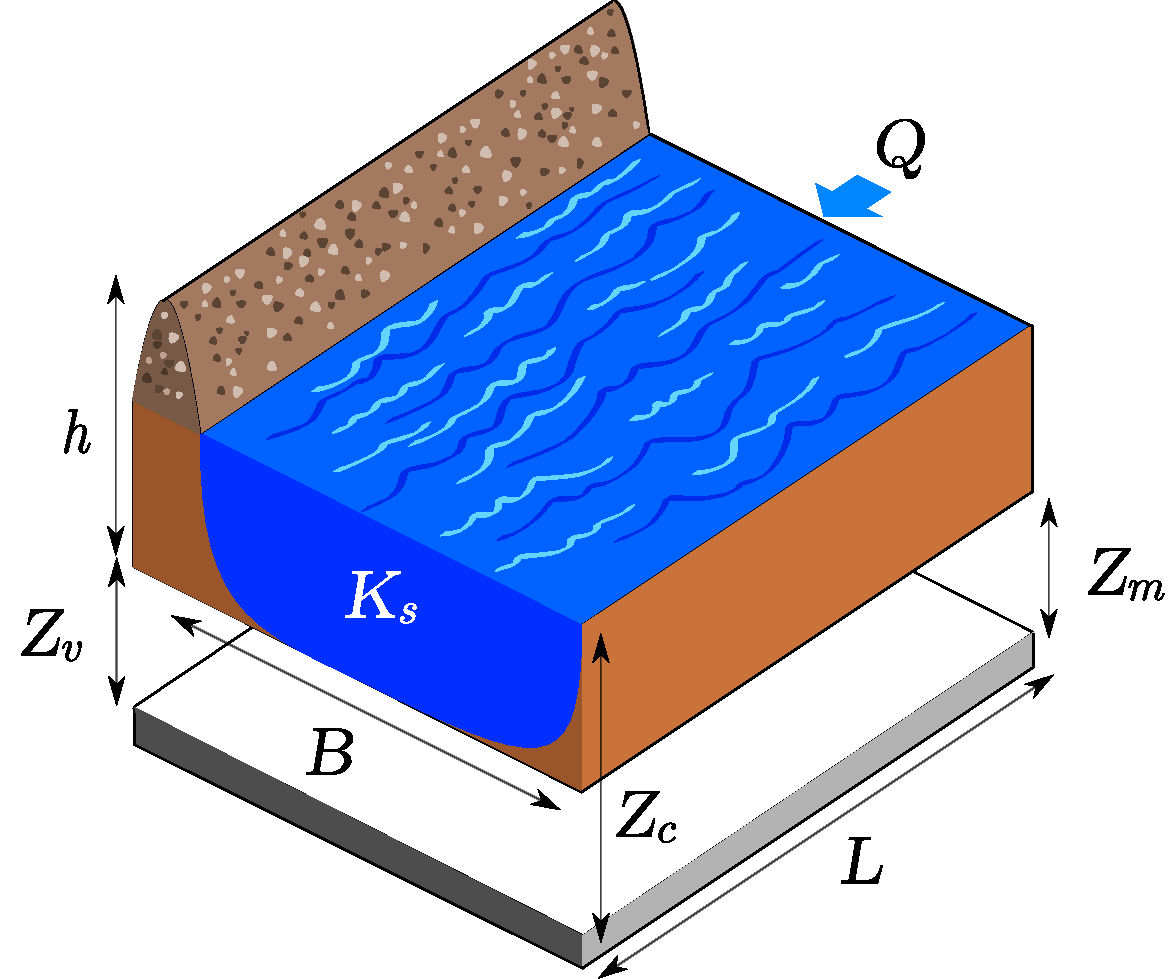
\includegraphics[width=9cm]{figures/river_section_large_adjusted} 
\end{center}
\caption{The flood example: simplified model of a river.}\label{fig:crues}
\end{figure}

\begin{table}[!ht]
  \begin{center}
   \begin{tabular}{lccc}
Input & Description & Unit & Probability distribution \\
   \hline
 $Q$ & Maximal annual flowrate & m$^3$/s & Gumbel ${\mathcal G}(scale = 558, mode = 1013)$ \\
 $K_s$ & Strickler coefficient & - & Normal ${\mathcal N}(30, 7.5)$  \\
 $Z_v$ & River downstream level & m & Uniform  ${\mathcal U}(49, 51)$ \\
 $Z_m$ & River upstream level  & m  & Uniform  ${\mathcal U}(54, 56)$\\
\hline
    \end{tabular}
    \caption{Input variables of the flood model and their probability distributions.}
    \label{tab:factors}
  \end{center}
\end{table}

The goal of this study is twofold:
\begin{itemize}
\item we want to estimate the mean river height $E(S)$, 
\item we want to perform the sensitivity analysis of the model, i.e. 
we want to rank the inputs $Q$, $K_s$, $Z_v$ and $Z_m$ with respect to their contributions 
to the variability of the output $S$.
\end{itemize}

%%%%%%%%%%%%%%%%%%%%%%%%%%%%%%%%%%%%%%%%%%%%%%%%%

\subsection{Define the random vector}

In this section, we present the Python script which allows to define the 
output random vector in OpenTURNS. 

We begin by importing the required modules.
\lstset{language=Python}
\begin{lstlisting}
from openturns.viewer import View
import openturns as ot
from math import sqrt
import pylab as pl
\end{lstlisting}


We first define the function through which we want to propagate the 
uncertainties with the \pyobj{def} operator.

\lstset{language=Python}
\begin{lstlisting}
def functionFlood(X) :
    Hd = 3.0
    Zb = 55.5
    L = 5.0e3
    B = 300.0
    Zd = Zb + Hd
    Q, Ks, Zv, Zm = X
    alpha = (Zm - Zv)/L
    H = (Q/(Ks*B*sqrt(alpha)))**(3.0/5.0)
    S = H + Zv
    return [S]
\end{lstlisting}

Then we convert this Python function into an OpenTURNS function with the 
\pyobj{Python\-Function} class. 

\lstset{language=Python}
\begin{lstlisting}
input_dimension = 4
g = ot.PythonFunction(input_dimension, 1, functionFlood)
\end{lstlisting}

Now we create the distributions for the input variables.
\begin{itemize}
\item There are several ways to set the parameters of the Gumbel distribution for the $Q$ variable. 
Here the parameters are defined with the scale and mode parameters, which corresponds to the 
\pyobj{GumbelAB} class.
\item The $Q$ and $K_s$ variables must remain positive (a negative value is not compatible with the 
physical model). 
For this reason, we must truncate the distribution with 
\pyobj{TruncatedDistribution}.
\end{itemize}

\begin{lstlisting}
myParam = ot.GumbelAB(1013., 558.)
Q = ot.ParametrizedDistribution(myParam)
otLOW = ot.TruncatedDistribution.LOWER
Q = ot.TruncatedDistribution(Q, 0, otLOW)
Ks = ot.Normal(30.0, 7.5)
Ks = ot.TruncatedDistribution(Ks, 0, otLOW)
Zv = ot.Uniform(49.0, 51.0)
Zm = ot.Uniform(54.0, 56.0)
\end{lstlisting}

We set the descriptions of the random variables: they are used for the graphics.
\begin{lstlisting}
Q.setDescription(["$Q (m^3/s)$"])
Ks.setDescription(["$Ks (m^{1/3})/s)$"])
Zv.setDescription(["Zv (m)"])
Zm.setDescription(["Zm (m)"])
\end{lstlisting}

The \pyobj{drawPDF} method plots the the probability distribution function of the variable. 
\begin{lstlisting}
Q.drawPDF()
\end{lstlisting}
The previous session produces the figure \ref{fig-variableQ}.
When we closely look at the PDF of $Q$, we see a small increase of the density for $Q=0$, because of the 
truncation of the distribution.


\begin{figure}
\centering
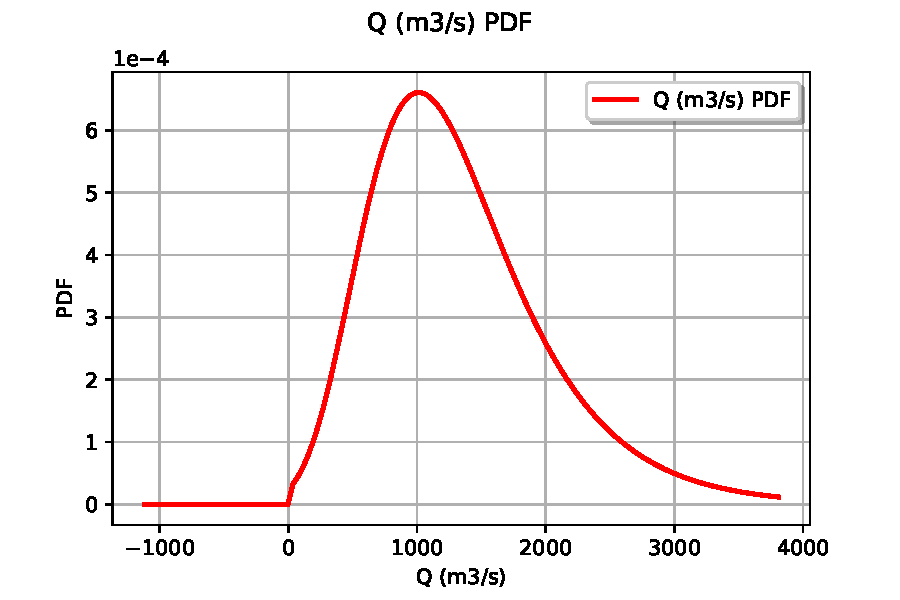
\includegraphics[width=0.8\textwidth]{figures/inputVariableQ.pdf}
\caption{The probability density function of the variable $Q$.}
\label{fig-variableQ}
\end{figure}

Then we create the input random vector \pyobj{inputvector}: by default, the copula is independent. 
Finally, we create the output random vector \pyobj{S}.
\begin{lstlisting}
X = ot.ComposedDistribution([Q, Ks, Zv, Zm])
inputRV = ot.RandomVector(X)
S = ot.RandomVector(g, inputRV)
\end{lstlisting}

These steps are typical of \emph{probabilistic programming}: we 
have defined the random variables involved in the problem 
\emph{without} having generating a sample so far.

%%%%%%%%%%%%%%%%%%%%%%%%%%%%%%%%%%%%%%%%%%%%%%%%%

\section{Estimating the mean with an incremental algorithm}

%%%%%%%%%%%%%%%%%%%%%%%%%%%%%%%%%%%%%%%%%%%%%%%%%

\subsection{Theory}

In this section, we present the principles that are used in a new incremental 
algorithm in OpenTURNS 1.12; the goal of this algorithm is to estimate the mean of a random variable. 
Moreover, we would like to let the user as free as possible from the internal details of the algorithm 
and get the best possible performance on a supercomputer.

Assume that the output $Y\in\mathbb{R}^{n_Y}$ is a random vector and that we want to estimate the 
mean $E(Y_i)$ for $i=1,...,n_Y$. 

The Monte Carlo method is based on the the sample mean: 
$$
\mu_i = \frac{1}{n} \sum_{j=1}^n Y_j^{(i)}
$$
for $i=1,...,n_Y$ where $n$ is the sample size and $Y_j^{(i)}$ are i.i.d. outcomes of the random output. 

The algorithm is based on the fact that the sample mean is asymptotically gaussian:
$$
\mu_i \sim \mathcal{N}\left(E(Y_i),\frac{V(Y_i)}{n}\right).
$$
for $i=1,...,n_Y$ where $V(Y_i)$ is the variance of the i-th output and $n$ is the sample size.

In general, most users set the sample size $n$ in advance and estimate the precision afterwards. 
Let $s_i$ be the (unbiased) sample standard deviation of the output $Y_i$:
$$
s_i = \sqrt{\frac{1}{n-1} \sum_{j=1}^N (y_j^{(i)}-\mu_i)^2}
$$
for $i=1,...,n_Y$. 
The absolute precision of the estimate $\mu_i$ can be estimated based on the sample standard deviation of the estimator:
$$
\sigma_i = \frac{s_i}{\sqrt{n}}
$$
for $i=1,...,n_Y$. 
If $\mu_i\neq 0$ and if $E(Y_i)\neq 0$, the relative precision can 
be estimated based on the coefficient of variation $\sigma_i/\mu_i$ 
for $i=1,...,n_Y$. 
 
Instead, suppose that we set the absolute precision in advance and wish to determine the smallest sample 
size $n$ that achieves this precision. 
If the variance $V(Y_i)$ is known (which rarely happens in practice), we can set the value of $n$ 
so that the standard deviation $\sqrt{V(Y_i)}$ is small enough. 
In the case where we want to set the relative precision, we can consider the coefficient of variation 
of the estimator $\frac{\sqrt{V(Y_i)}}{E(Y_i)\sqrt{n}}$ as a criterion (if $E(Y_i)\neq 0$). 
However, we generally do not know the values of neither $E(Y_i)$ nor $V(Y_i)$. 
This is why setting the sample size $n$ in advance is not an easy task for the 
user in general. 

The purpose of the algorithm is to increase the 
sample size $n$ incrementally until a stopping criteria is met. 
At each iteration, we approximate the values of $E(Y_i)$ and $V(Y_i)$ 
by their empirical estimators, which allows to evaluate the stopping criteria. 

In order to get the best possible performance on distributed supercomputers and 
multi-core workstations, the size of the sample increases by block. 
For exemple, if the block size is equal to 100, then the sample size will be equal to 0, 100, 
200, etc... 
On each block, the evaluation of the outputs can be parallelized, which allows to improve the 
performance of the algorithm.
More details on this topic are presented in the section \ref{sec-hpceasy}. 

Since there are in general several outputs, i.e. $n_Y\geq 1$, we use 
a stopping criteria which is based on a operator. 
There are three mathematical stopping criteria available:
\begin{itemize} 
\item through an operator on the coefficient of variation $\frac{\sigma_i}{\mu_i}$ (a relative criterion),
\item through an operator on the standard deviation $\sigma_i$ (absolute criterion),
\item on the maximum standard deviation per component: $\sigma_i \leq \max_{i=1,...,n_Y} \sigma_i$ (absolute criterion).
\end{itemize} 

By default, the maximum coefficient of variation is used, i.e. the operator is the \emph{maximum} 
so that the algorithm stops when: 
$$
\max_{i=1,...,n_Y} \frac{\sigma_i}{\mu_i} \leq max_{COV}.
$$
%%%%%%%%%%%%%%%%%%%%%%%%%%%%%%%%%%%%%%%%%%%%%%%%%

\subsection{Tutorial}

In this section, we present how to use the \pyobj{ExpectationSimulationAlgorithm} class 
in the tutorial flooding example. 
We set the maximum number of iterations with the \pyobj{setMaximum\-OuterSampling} so that 
we use at most 1000 iterations. 
In order to evaluate the function with blocks of size 10, we use the \pyobj{setBlockSize}. 
In this simulation, we use a relative stopping criteria and configure the 
maximum coefficient of variation to be equal to 0.001.
\begin{lstlisting}
algo = ot.ExpectationSimulationAlgorithm(S)
algo.setMaximumOuterSampling(1000)
algo.setBlockSize(10)
algo.setMaximumCoefficientOfVariation(0.001)
\end{lstlisting}
The computationnaly intensive part of the simulation is associated with the 
\pyobj{run} method. 
\begin{lstlisting}
algo.run()
\end{lstlisting}
Once the simulation is done, the \pyobj{getResult} method allows to 
access to the results.
\begin{lstlisting}
result = algo.getResult()
expectation = result.getExpectationEstimate()
print("Mean = %f " % expectation[0])
print("Number of calls to G = %d" % g.getCallsNumber())
\end{lstlisting}
The previous session prints the following output.
\begin{lstlisting}
Mean = 52.520729 
Number of calls to G = 500
Coef. of var.=0.000994
\end{lstlisting}
The estimate of the mean has a known asymptotical gaussian distribution, which can be retrieved 
with the \pyobj{getExpectation\-Distribution} method.
\begin{lstlisting}
expectationDistribution = result.getExpectationDistribution()
print(expectationDistribution)
View(expectationDistribution.drawPDF())
\end{lstlisting}
We emphasize that the output of the \pyobj{getExpectation\-Distribution} method is 
a \pyobj{Distribu\-tion} in the OpenTURNS sense: the whole information is available, 
not just a part of it, making the output as programmatically meaningful as possible. 
\begin{lstlisting}
expectationDistribution = result.getExpectationDistribution()
expectationDistribution.drawPDF()
\end{lstlisting}
The previous script produces the figure \ref{fig-variableMeanS}. 
The figure shows that we have an accurate estimate of the mean, 
up to approximately 2 significant digits. 

\begin{figure}
\centering
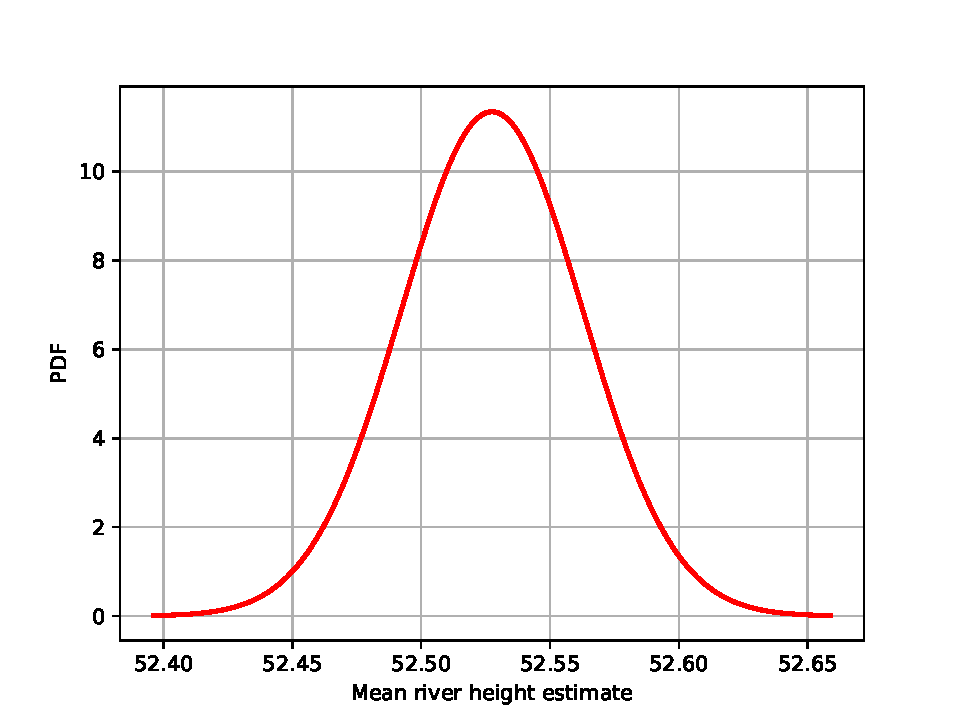
\includegraphics[width=0.8\textwidth]{figures/MeanSDistribution.pdf}
\caption{The probability density function of the estimate 
of the mean of the river height.}
\label{fig-variableMeanS}
\end{figure}

%%%%%%%%%%%%%%%%%%%%%%%%%%%%%%%%%%%%%%%%%%%%%%%%%

\section{Estimate sensitivity indices with an incremental algorithm}

\subsection{Theory}

In this section, we present the principles that are used in a new incremental 
algorithm in OpenTURNS 1.12 which computes the Sobol' sensitivity indices. 

In \cite{Janon2014} the authors derive a new method to estimate the 
Sobol' sensitivity indices ; one of the advantages of the new 
estimator is that it is associated with an asymptotic distribution, 
which is derived thanks to the so called "delta"-method. 
Based on a suggestion by R.Lebrun, A. Dumas \cite{RapportSobol2018} 
used the same theoretical method in order to derive the 
asymptotic distribution of Sobol' sensitivity indices already available 
in OpenTURNS. 

%%%%%%%%%%%%%%%%%%%%%%%%%%%%%%%%%%%%%%%%%%%%%%%%%

\subsubsection{Overview}

Let us denote by $X\in\mathbb{R}^{n_X}$ a random vector. 
This algorithm works in the general case where the output $Y\in\mathbb{R}^{n_Y}$ is a random 
vector: in this case it operates on aggregated indices. 
In order to simplify the discussion, let us make the hypothesis that $n_Y=1$. 

The Sobol' first order sensitivity indices are defined by 
$$
S_i = \frac{V(E(Y|X_i))}{V(Y)}
$$
for $i=1,...,n_X$. The total order sensitivity indices are defined by :
$$
T_i = 1 - \frac{V\left(E\left(Y|X_{-i}\right)\right)}{V(Y)}
$$
where $-i$ is the set of indices which are different from $i$. 
In the remaining of this section, 
we focus on the first order sensitivity indice and let the reader consider [1] for the total 
order indices. 
Moreover, the derivation is the same for all input variables so that we omit the 
indice $i$ in order to simplify the notations. 

%%%%%%%%%%%%%%%%%%%%%%%%%%%%%%%%%%%%%%%%%%%%%%%%%

\subsubsection{Asymptotic distribution}

The algorithm is based on the fact that the estimators of the 
first and total order Sobol' sensitivity indices 
asymptotically have the gaussian distribution. 
This gaussian distribution can be derived from the 
so called "delta"-method. 

Assume that the Sobol' estimator is 
$$
\overline{S} = \Psi\left(\overline{U}\right)
$$
where $\Psi$ is a multivariate function, $U$ is a multivariate sample and $\overline{U}$ is its 
sample mean. 
Each Sobol' estimator can be associated with a dedicated choice of function $\Psi$ 
and vector $U$. 

Let us denote by $\Phi_j^F$ (resp. $\Phi_j^T$) the cumulated distribution function of the 
gaussian distribution of the first (resp. total) order sensitivity indice of the j-th input 
variable.

Each available estimator in the library provides its own distribution, namely 
the Saltelli, Mauntz-Kucherenko, Jansen and Martinez estimators.

%%%%%%%%%%%%%%%%%%%%%%%%%%%%%%%%%%%%%%%%%%%%%%%%%
\subsubsection{Stopping criteria}

We set $\alpha\in[0,1]$ the level of the confidence interval and $\epsilon \in(0,1]$ the length 
of the confidence interval. 
The algorithms stops when, on all components, one of the two 
following conditions are satisfied :
\begin{itemize}
\item first and total order indices haved been estimated with enough precision or 
\item the first order indices are separable from the total order indices. 
\end{itemize}

The precision is said to be sufficient if the $1-2\alpha$ confidence interval is smaller than 
$\epsilon$ :
$$
(\Phi_j^F)^{-1}(1-\alpha) - (\Phi_j^F)^{-1}(\alpha) \leq \epsilon
$$
and 
$$
(\Phi_j^T)^{-1}(1-\alpha) - (\Phi_j^T)^{-1}(\alpha) \leq \epsilon
$$
for $j=1,...,n_X$.  
The first order indices are \emph{separable} from the total order indices if 
$$
\Phi_j^F(1-\alpha) \leq \Phi_j^T(\alpha)
$$
for $j=1,...,n_X$.  
This criteria allows to stop when the algorithm has detected an interaction 
between input variables with sufficient precision. 

%%%%%%%%%%%%%%%%%%%%%%%%%%%%%%%%%%%%%%%%%%%%%%%%%

\subsection{Tutorial}

In this section, we present how to use the \pyobj{SaltelliSensitivityAlgorithm} classe 
in the tutorial flooding example. 


We first set the parameters of the algoritms. 
We set the \pyobj{alpha} variable so that a 90\% confidence interval is used. 
In order to get confidence intervals which are not greater than 0.2, we set 
the variable \pyobj{epsilon} variable accordingly. 
The block size corresponds to the size of the Sobol' design of experiment generated 
at each iteration. 
Finally, the \pyobj{batchsize} variable contains the number of points evaluated simultaneously 
by the model. 
\begin{lstlisting}
alpha = 0.05 # 90% confidence interval
epsilon = 0.2 # Confidence interval length
blocksize = 50 # Size of Sobol experiment at each iteration
batchsize = 16 # Number of points evaluated simultaneously
\end{lstlisting}

Then we create the algorithm and configure the algorithm so that it 
uses the previous variables. 
Moreover, we configure the algorithm so that at most 100 iterations are used. 
\begin{lstlisting}
estimator = ot.SaltelliSensitivityAlgorithm()
estimator.setUseAsymptoticDistribution(True)
algo = ot.SobolSimulationAlgorithm(X, g, estimator)
algo.setMaximumOuterSampling(100) # number of iterations
algo.setBlockSize(blocksize) 
algo.setBatchSize(batchsize) 
algo.setIndexQuantileLevel(alpha) # alpha
algo.setIndexQuantileEpsilon(epsilon) # epsilon
algo.run()
\end{lstlisting}

Once that the algorithm has run, the results can be retrieved and estimates 
of first and total order indices can be printed. 
\begin{lstlisting}
result = algo.getResult()
fo = result.getFirstOrderIndicesEstimate()
to = result.getTotalOrderIndicesEstimate()
print("First order = %s" % (str(fo)))
print("Total order = %s" % (str(to)))
\end{lstlisting}

The previous script produces the following output.
\begin{lstlisting}
First order = [0.529059,0.205321,0.381215,0.0316592]
Total order = [0.481355,0.130565,0.362292,0.011206]
\end{lstlisting}

We can obtain the asymptotic distribution of the first and total 
order indices. 
For example, the following script extracts the first component of the 
asymptotic distribution of the first order indice (which corresponds to the variable 
$Q$) and plots it.
\begin{lstlisting}
dist_fo = result.getFirstOrderIndicesDistribution()
dist_fo_i = dist_fo.getMarginal(0)
graph = dist_fo_i.drawPDF()
graph.setTitle("S0")
graph.setXTitle("S0")
\end{lstlisting}
The previous script produces the figure \ref{fig:asymptQ}.

\begin{figure}[!ht]
\begin{center}
    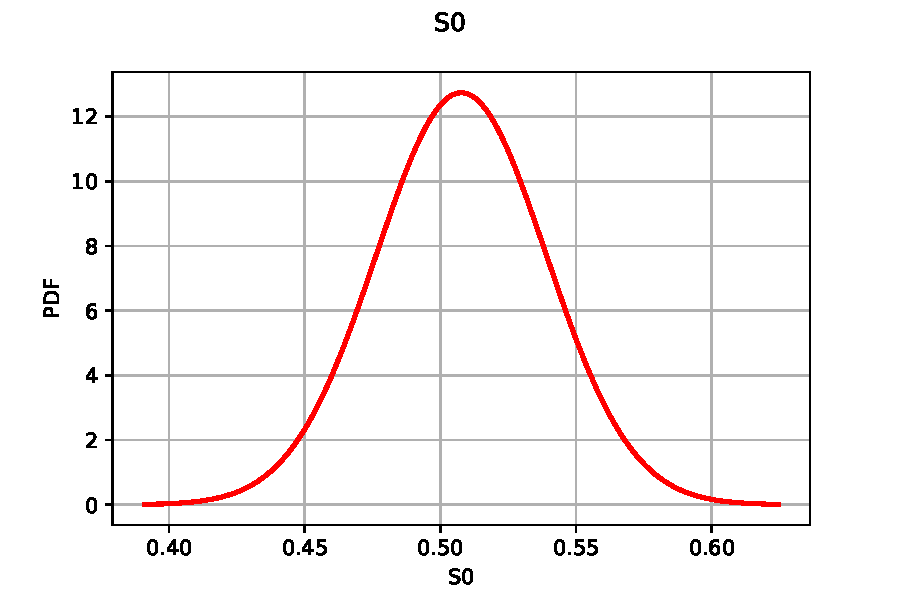
\includegraphics[width=9cm]{figures/S0-distribution} 
\end{center}
\caption{Asymptotic distribution of the first order Sobol' indices 
for the $Q$ variable.}
\label{fig:asymptQ}
\end{figure}

In order to get a more compact view of the first and total order indices 
along with their confidence intervals, we often represent the 90\% confidence 
intervals with a vertical bar. 
The figure \ref{fig:sobolindices} presents the Sobol' indices with 
asymptotic confidence intervals. 
We observe that the the confidence intervals are relatively small, 
as expected. 

\begin{figure}
\begin{center}
    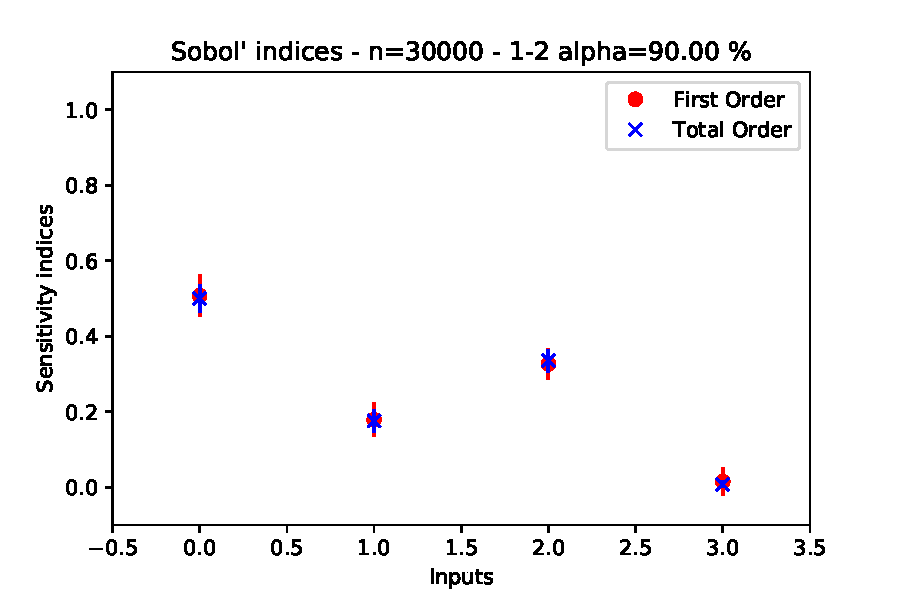
\includegraphics[width=9cm]{figures/crue-Sobol-indices} 
\end{center}
\caption{Sobol' indices with asymptotic confidence intervals.}
\label{fig:sobolindices}
\end{figure}

%%%%%%%%%%%%%%%%%%%%%%%%%%%%%%%%%%%%%%%%%%%%%%%%%

\section{New features in the graphical user interface}

\subsection{Introduction}

There are situations where the engineer in charge of performing an uncertainty study does not want to use
a programming language such as C++ or Python. 
In this context, providing a graphical user interface (GUI) may allow to greatly increase the use of
OpenTURNS and, more generally, of the UQ methodology. 

This is why we develop since 2016 a graphical user interface (GUI) of OpenTURNS, which is integrated within 
SALOME \cite{SALOMEurl}. 
This GUI is developed with the OpenSource LGPL license, which is the same as OpenTURNS and SALOME. 
SALOME binaries for the Linux platform are provided at the following URL:
\begin{center}
\url{https://www.salome-platform.org/contributions/edf_products}
\end{center}
Details on the main features and the internal architecture of the GUI were already presented in \cite{OpenTURNSUncecomp17}, 
this is why this paper focuses on the new features. 

%%%%%%%%%%%%%%%%%%%%%%%%%%%%%%%%%%%%%%%%%%%%%%%%%

\subsection{Dependency structures}

The GUI allows to define advanced dependency structures, based on copulas. 
The figure \ref{fig-copula} presents the dialog box in which the copulas can be selected and 
configured. 

\begin{figure}
\centering
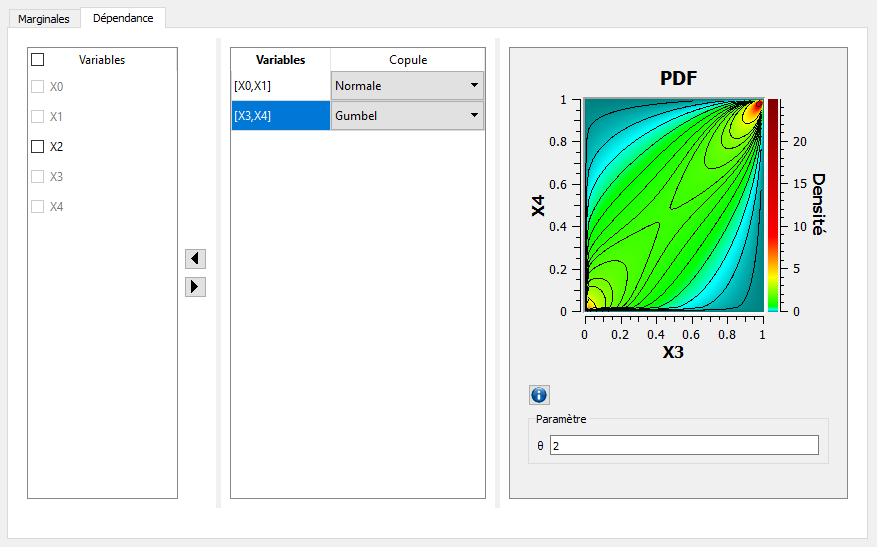
\includegraphics[width=\textwidth]{figures/capture-otgui-copule-focus.png}
\caption{Managing a copula in the OpenTURNS GUI.}
\label{fig-copula}
\end{figure}

The principle is to create sub-groups within the input variables. 
Within a given sub-group, we can select the copula and configure its parameters. 
Seven copulas are available: independent, Gaussian, Ali-Mikhail-Hak, Clayton, 
Farlie-Gumbel-Morgensten, Frank or an inference result.  

For example, the figure \ref{fig-copula} considers the situation in which the model has 
five inputs named X0, X1, X2, X3 and X4. 
In this particular model, the sub-group [X0,X1] is associated with the Gaussian copula while the 
sub-group [X3,X4] is associated with the Gumbel copula. 
The variable X2 remains independent from the others in this model. 

Moreover, any multivariate sample can be used to estimate the parameters of a 
copula. 
This is case, the results of an inference can be reused in a dependency model. 

%%%%%%%%%%%%%%%%%%%%%%%%%%%%%%%%%%%%%%%%%%%%%%%%%

\subsection{Screening with the Morris method}

The qualitative sensitivity analysis based on Morris's method \cite{Morris1991} aims at 
selecting the significant input variables in a costly computer code which may have 
a large number of inputs. 
The GUI performs the screening analysis based on the OpenTURNS \pyobj{otmorris} module \cite{otmorris}. 

Let $e_i^k$ be the k-th computed elementary effects associated to the i-th input marginal, 
the method computes $\mu_i^*$ and $\sigma_i$ respectively the absolute mean and the standard deviation of the elementary effects. 
The goal of this method is to set the inputs variables into three classes, based on $\mu_i^*$ 
and the $\rho_i = \frac{\mu_i^*}{\sigma_i}$ factors:
\begin{enumerate}
\item if $\mu_i^*$ is close to zero, the i-th variable has no effect,
\item if $\rho_i \leq 0.5$ the i-th variable has almost linear effects,
\item if $\rho_i \geq 1$ the i-th variable has non-linear and non-monotonic effects
\end{enumerate}

The figure \ref{fig-morris} presents the dialog box which contains the parameters of the 
algorithm. 
The user can set the number of trajectories and the number of levels for each variable. 
The dialog box automatically computes the corresponding number of simulations and prints 
it in the bottom of the dialog box. 

\begin{figure}
\centering
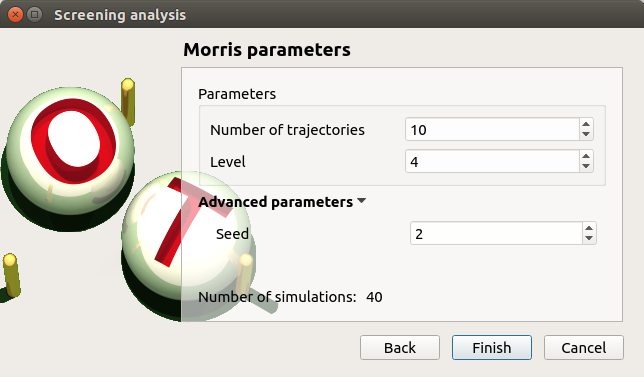
\includegraphics[width=0.7\textwidth]{figures/morris_wizard_3rd_page.png}
\caption{Performing screening with Morris's method in the GUI.}
\label{fig-morris}
\end{figure}

Once the simulations are performed, the figure \ref{fig-morrisresultats} presents the results 
associated with a physical model which has 20 input variables. 
The main figure presents the mean and standard deviations of the elementary effects. 
A table (not shown in the figure) containing the list of input variables allows 
to see in which category fall each variable. 
A default classification is done by the GUI, but can be modified by the user. 

\begin{figure}
\centering
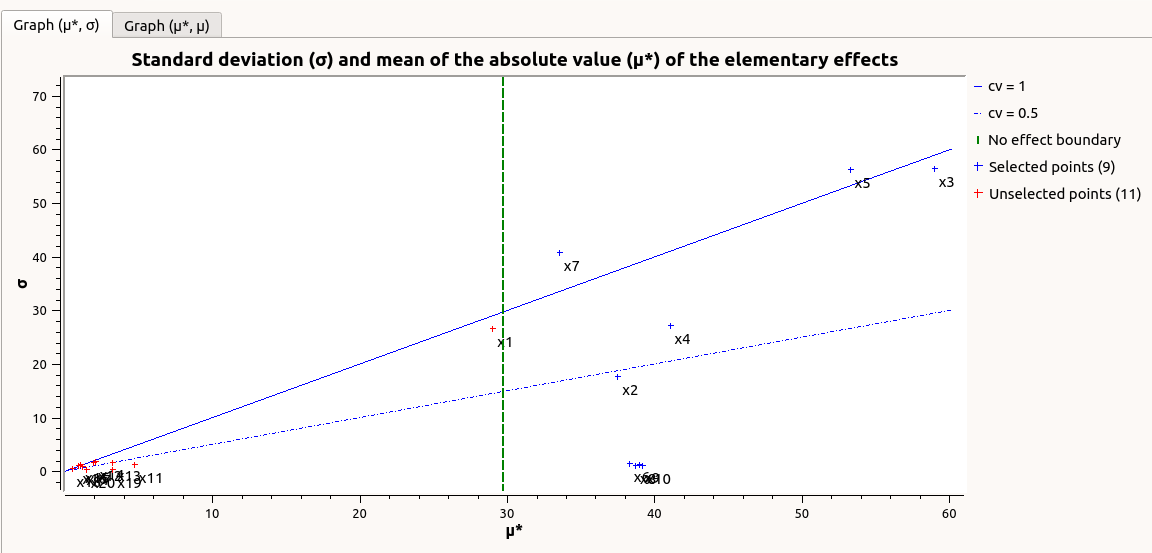
\includegraphics[width=\textwidth]{figures/morrisResultWindow-up.png}
\caption{Results of the screening with Morris's method in the GUI.}
\label{fig-morrisresultats}
\end{figure}

%%%%%%%%%%%%%%%%%%%%%%%%%%%%%%%%%%%%%%%%%%%%%%%%%

\subsection{Easy high performance computing}
\label{sec-hpceasy}

Within SALOME, users can access to the remote high performance computing 
resources available at EDF R\&D. 
Based on 16 100 cores, the Porthos supercomputer (2014) for example, can perform as high as 600Tflops (peak) \cite{Top500Porthos}. 
The latest supercomputer at EDF R\&D, Gaïa (2019), can perform as high as 3 052 Tflops (peak) \cite{Top500Gaia} 
thanks to its 41 000 cores. 

Within the GUI, the user can run simulations which are executed on a remote supercomputer with 
a minimum amount of configuration. 
The figure \ref{fig-hpcsalome} presents the dialog box which is displayed in the 
context of a central tendency study based on a Monte-Carlo simulation. 
Enabling the \emph{Parallelize status} checkbutton allows to select the 
computing resource available in the users environment. 
The number of processes can be chosen by the user according to the hardware available 
and the amount of computing required by the simulation. 
Each job is associated with a time limit which defines the maximum 
duration of one job. 
In most practical situations extra input files are used by the computer code (e.g. the mesh), 
which can be configured in the dialog box as well. 
The job submission is based on SLURM, but the user does not have to configure these 
low-level parameters which are handled automatically by the algorithms, with the principles 
which we now present. 

\begin{figure}
\centering
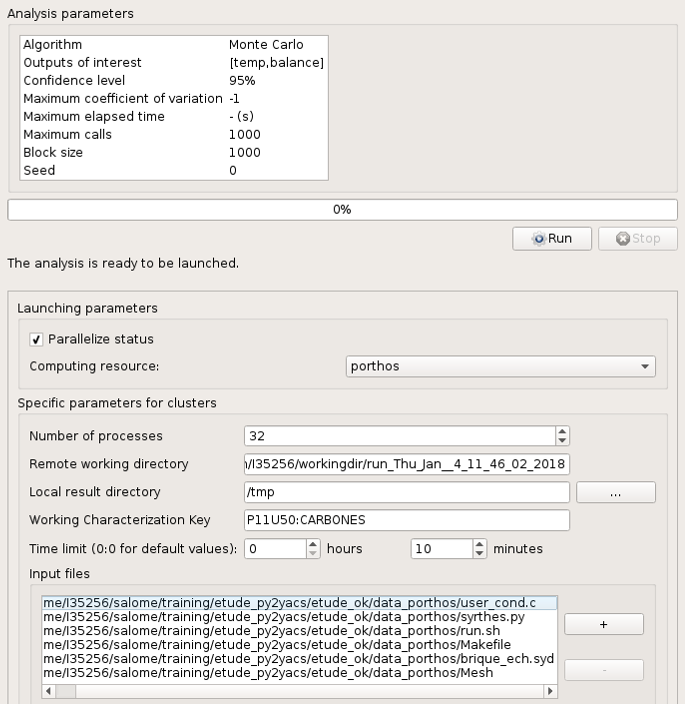
\includegraphics[width=\textwidth]{figures/SALOME-OpenTURNS-config-HPC-focus.png}
\caption{Launching a parallel computation within the GUI.}
\label{fig-hpcsalome}
\end{figure}

The key point is to exploit the maximum possible amount of parallelism in 
the computations. 
However, between the start of the simulation and the end (which might take minutes, hours 
or days in the longest situations), most users want to regularily have a feedback on the 
execution of the simulation. 
For these reasons, the algorithms are performed based on blocks, which define a sub-sample 
on which the parallel computation can take place. 
At the end of each block, a progress bar is updated along with statistics which shows the 
number of executed simulations, the elapsed time and the value of the stopping criteria 
(e.g. the coefficient of variation of the mean estimator). 
A \emph{Stop} button allows to interrupt the simulation. 

Consider for example the situation presented in the figure \ref{fig-blockalgo}, 
where a design of experiments involving 24 points must be evaluated. 
The parameters configured by the user in this example is the size of the block, which is set 
to 12, and the number of processors, which is set to 4. 
In this case, the simulation starts with a first job involving the points with indices from 1 to 12, 
and ends with a second job involving the points with indices 13 to 24. 
In both jobs, each processor is in charge of the evaluation of three points. 

\begin{figure}
\centering
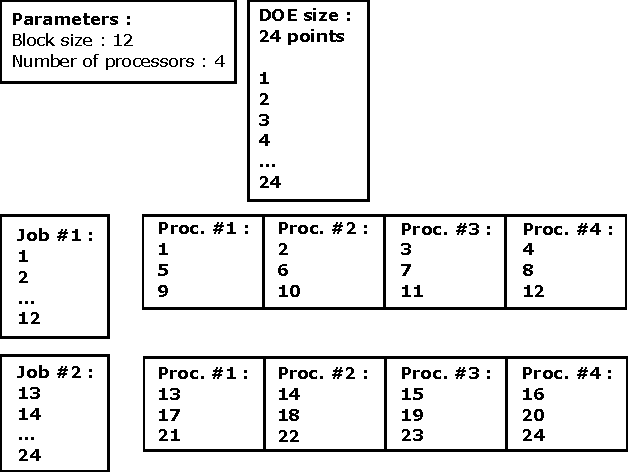
\includegraphics[width=0.5\textwidth]{figures/SALOME-OpenTURNS-simulation-byblock.pdf}
\caption{A block-based simulation performed on a supercomputer using two jobs.}
\label{fig-blockalgo}
\end{figure}


%%%%%%%%%%%%%%%%%%%%%%%%%%%%%%%%%%%%%%%%%%%%%%%%%

\subsection{Perspectives: one-dimensional stochastic processes}

In this section, we present the current developments of the GUI, which focuses on the 
management on stochastic fields. 

Indeed, there are various situations in which the simulator through which we propagate the 
uncertainties produces a stochastic process. 
This happens for example in the case where the simulator produces a time series or 
a one-dimensional spatial field. 

The figure \ref{fig-trajectories} presents a set of trajectories in the GUI. 
In general, the sample size is large and this graphics does not convey much information, 
because the trajectories overlap and hide each other. 

\begin{figure}
\centering
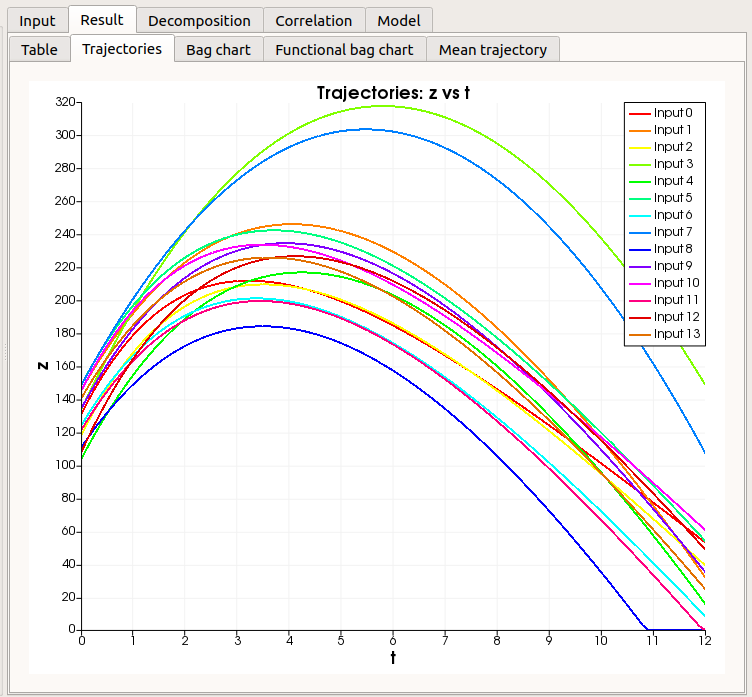
\includegraphics[width=\textwidth]{figures/central_tendency_trajectories-focus.png}
\caption{A sample set of trajectories in the GUI.}
\label{fig-trajectories}
\end{figure}

Obviously, this situation is more complex than the classical output random 
vector that many engineers are used to and require more advanced 
probabilistic methods. 
The most common way of managing such situation is to use a 
dimension reduction method such as the principal component analysis or the 
Karhunen-Loève decomposition. 

This is why Ribes et al \cite{Ribes2014} developed a new visualization tool in \cite{PVurl}, based on a 
work by Kitware. 
This tool is the \emph{functional bag chart}, also known as the highest density region 
plot in the bibliography. 
The figure \ref{fig-functionnalbagchart} presents the functional bag chart of a sample 
set of trajectories. 
This graphics allows to plot a functional boxplot in the sense that it plots a functional 95\% confidence 
region. 
The graphics also allows to detect outlier trajectories, i.e. trajectories which achieve a low 
density in the reduced space. 

\begin{figure}
\centering
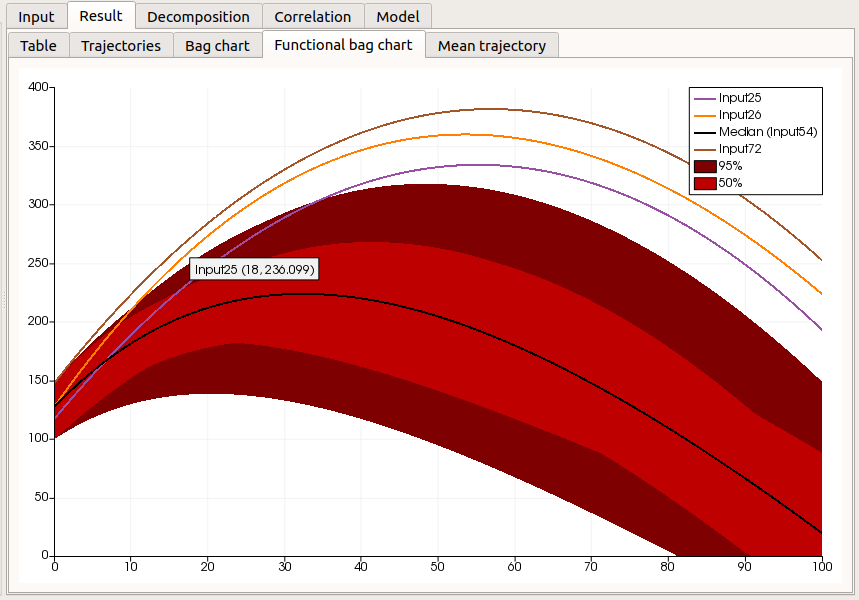
\includegraphics[width=\textwidth]{figures/functional_bag_chart-focus.png}
\caption{The functional bag chart of Paraview to plot a functional boxplot and detect outlier trajectories.}
\label{fig-functionnalbagchart}
\end{figure}

The future version will extend these functional analyses to higher dimensions, including 2D stochastic fields. 

%%%%%%%%%%%%%%%%%%%%%%%%%%%%%%%%%%%%%%%%%%%%%%%%%%%%%%%%%%%%%%%%%%%%%%

\bibliographystyle{plain}
\bibliography{otgui}


%%%%%%%%%%%%%%%%%%%%%%%%%%%%%%%%%%%%%%%%%%%%%%%%%%%%%%%%%%%%%%%%%%%%%%

\end{document}
